%% Languages: norsk				
%%						english			
%% Styles:		twoside, 		The margins will differ dependent on right/left pages
%%						openright		The first page is a "right" page
%% indexes:		listings		Show figure list, table list
%%						glossary		Show glossary and abbreviation list
%%						todo				Show list of todo-notes in documents
%%						%
\documentclass[english]{gucreport}
%% 'gucreport.cls' - a LaTeX class for reports at GUC, based upon gucthesis.cls
%%
%% Copyright (C) 2014 Magnus �verb�
%% 'gucthesis.cls' - Copyright (C) 2005 Ivar Farup and Kjetil Orbekk
%%
%% CHANGE LOG:
%%
%% v0.1 2005/03/09:
%%  * First pre-alpha draft
%%
%% v0.2 2005/03/10:
%%  * Reduced size of heading to 7pt
%%  * Reimplemented the heading without using fancyhdr, making the
%%    package (more) compatible with hyperref.
%%  * Introduced \thesisdate for upper right header
%%
%% v0.3 2005/03/11:
%%  * \chapter{} and \chapter*{} heading can cover several lines
%%
%% v0.4 2005/04/19:
%%  * new itemize and enumerate environments
%%  * twoside, adjusted headers and margins; header and footers are
%%    not shown on pages that are empty due to new chapters
%%  * \thesistitlepage: dummy title page using new commands
%%    \thesisauthor, \thesisdate, and \thesistitle
%%  * no centering of sections
%%  * \subsubsection and \paragraph now produce an error message
%%
%% v0.5 2005/05/10:
%%  * \subsubsection and \paragraph reintroduced
%%  * \parskip and \parindent changed
%%
%% v0.6 2005/05/13:
%%  * \chapter no longer in capitals
%%
%% v0.7 2007/05/30:
%%  * Added frontpage matter implemented by Kjetil Orbekk
%% 'gucmasterthesis.cls' - a LaTeX class for master's theses at GUC
%%
%%
%% 2014/02/06
%%	* Removed redundant code from creating front pages
%%	* Specific types of study programs are more easily created
%%	* Added a separate counter for wordcount
%%	* Added a second title page for bachelor students
%%	* Fixed norwegian/english language bug
%%	*	Fixed cleardoublepage on summaries on twoside
%%
%% 2014/02/23
%%	* Created report template with frontpage 
%%	* 
%%	* 
%%

%%	Fix norsk option, since it returns errors on UTF8x
%%	
%%	
%%	


%%	IF
\newif\if@norsk
	\@norskfalse
\newif\if@english
	\@englishtrue
\newif\if@showIndex
	\@showIndexfalse
\newif\if@showDict
	\@showDictfalse
\newif\if@showTodo
	\@showTodofalse

%% IDENTIFICATION
\xdef\gucrepd{2014/02/28}
\xdef\gucrepv{1.00.00}
\NeedsTeXFormat{LaTeX2e}
\ProvidesClass{gucreport}
  [\gucrepd\space
   v\gucrepv\space
   Copyright (C) 2014 Magnus �verb�.
	 Based on the gucthesis class by Ivar Farup and Simon McCallum]

%% CLASS FILE COMMANDS
\LoadClass[a4paper]{report}

%% PACKAGE LOADING
\RequirePackage{geometry}
\RequirePackage[T1]{fontenc}\RequirePackage[utf8x]{inputenc}
\RequirePackage[utf8x]{inputenc}
\RequirePackage{euler}
\RequirePackage{lastpage}
\RequirePackage{babel}
\RequirePackage[pdftex]{graphicx, hyperref}
\RequirePackage{color}
\RequirePackage{nomencl}
\RequirePackage{pdfpages}
\RequirePackage{multicol}
\RequirePackage{longtable}
\RequirePackage[table]{xcolor}
\RequirePackage[all]{hypcap}
\RequirePackage[xindy]{glossaries}
\RequirePackage{listings}
\RequirePackage{amsmath}
\RequirePackage{amssymb}
\RequirePackage{bbding}
\RequirePackage{caption}
\RequirePackage{todonotes}

%	Counters
\newcounter{firstchapter}       % hack to find out where to start
	\c@firstchapter=1             % arabic page numbering, see below
\newcounter{tmpfig}             % hack to have continuous numbering of
\newcounter{tmptab}             % figures and tables, see below
\newcounter{numapp}

\newcommand{\numberofapp}{%
	\immediate\write\@auxout%
	{\string\setcounter{numapp}{\the\c@chapter}}%
}

\newcommand{\pagespace}{
	\if@openright		\cleardoublepage
	\else						\clearpage
	\fi
}

%% OPTIONS (declare more here if needed)
\DeclareOption{norsk}{
	\@norsktrue \@englishfalse
}
\DeclareOption{english}{
	\@englishtrue	\@norskfalse
}
\DeclareOption{oneside}{
	\@twosidefalse \@mparswitchfalse%
	\geometry{a4paper, left=3.75cm, right=3.75cm, top=3cm, 
						bottom=4cm, head=1.2cm, foot=2cm}
}
\DeclareOption{twoside}{
	\@twosidetrue  \@mparswitchtrue%
	\geometry{a4paper, left=4.5cm, right=3cm, top=3cm, 
						bottom=4cm, head=1.2cm, foot=2cm}
}
\DeclareOption{listings}{
	\@showIndextrue
}
\DeclareOption{glossary}{
	\@showIndextrue
	\@showDicttrue
}
\DeclareOption{todo}{
	\@showIndextrue
	\@showTodotrue
}

%
%	CUSTOM CONFIG AND COMMANDS
\renewcommand*{\glspostdescription}{}
\renewcommand{\lstlistingname}{Code}
\renewcommand\lstlistlistingname{
	\if@norsk	Kodesnutter og skript	
	\else			Code snippets and scripts
	\fi
}
\newcommand{\comment}[1]{\textcolor{blue}{\emph{#1}}}	%	Comment
\newcommand{\com}[1]{{\color{red}#1}}									% Supervisory comment
\renewcommand{\todo}[1]{{\color{green}#1}}						% Items to do
\newcommand{\n}[1]{{\color{blue}#1}} 									% Other comment
\newcommand{\dn}[1]{} 																% Finished comment
\renewcommand{\nomname}{
	\if@norsk	Forkortelser	
	\else			List of Abbreviations
	\fi
}				%	Abbrevations

\renewcommand*{\nompreamble}{\begin{multicols}{2}}		%
\renewcommand*{\nompostamble}{\end{multicols}}				%
\setlength{\columnsep}{3em}														% 
\setlength{\nomitemsep}{0.01cm}												% 

\AtBeginDocument{
	\baselineskip=14pt%
  \parskip=0pt%
  \parindent=14pt%
  \frenchspacing%
  \setcounter{secnumdepth}{2}%
  \setcounter{tocdepth}{1}%
	\if@showIndex\if@showDict
		\makeglossaries		% Glossary
		\makenomenclature	% Abbreviations
	\fi\fi
}
\pagenumbering{roman}           % until first chapter, see below
\captionsetup{justification=centering}

% Header and footer
\def\wordcount{ wordcount }
	\def\wordcount#1{\def\wordcount{#1}}

\def\projtitle{ projtitle }
	\def\projtitle#1{\def\projtitle{#1}}

\def\projsubtitle{ projsubtitle }
	\def\projsubtitle#1{\def\projsubtitle{#1}}

\def\projdate{ projdate }
	\def\projdate#1{\def\projdate{#1}}

\def\keywords{ keywords }
	\def\keywords#1{\def\keywords{#1}}

\def\appnumber{ appnumber }
	\def\appnumber#1{\def\appnumber{#1}}

\def\pagecount{ LastPage  }
	\def\pagecount#1{\def\pagecount{#1}}

\def\projvers{projvers}
	\def\projvers#1{\def\projvers{#1}}

\def\projauthor{ projauthor }
	\def\projauthor#1{\def\projauthor{#1}}

\def\projauthorid{ projauthorid}
	\def\projauthorid#1{\def\projauthorid{#1}}

\def\projauthorAid{ projauthorid}
	\def\projauthorAid#1{\def\projauthorAid{#1}}
\def\projauthorA{ projauthor }
	\def\projauthorA#1{\def\projauthorA{#1}}

\def\projauthorBid{ projauthorid}
	\def\projauthorBid#1{\def\projauthorBid{#1}}
\def\projauthorB{ projauthor }
	\def\projauthorB#1{\def\projauthorB{#1}}

\def\projauthorCid{ projauthorid}
	\def\projauthorCid#1{\def\projauthorCid{#1}}
\def\projauthorC{ projauthor }
	\def\projauthorC#1{\def\projauthorC{#1}}

\def\projauthorDid{ projauthorid}
	\def\projauthorDid#1{\def\projauthorDid{#1}}
\def\projauthorD{ projauthor }
	\def\projauthorD#1{\def\projauthorD{#1}}

	\def\courseid{ courseid }
	\def\courseid#1{\def\courseid{#1}}
\def\coursename{ coursename }
	\def\coursename#1{\def\coursename{#1}}

\def\projteacher{ projteacher }
	\def\projteacher#1{\def\projteacher{#1}}

\def\keywords{ keywords }
	\def\keywords#1{\def\keywords{#1}}

%% Headings
\def\ps@gucheadings{%
	\def\@oddfoot{\reset@font \hfill \thepage/\pageref{LastPage} \hfill }
  \let\@evenfoot=\@oddfoot
  \def\@oddhead{
		\underline{
			\hbox to\hsize{
				\fontsize{8}{10}	\selectfont \hfill \projtitle \hfill
			}%hsize
		}%underline
	}%oddhead
  \let\@evenhead=\@oddhead
}
\pagestyle{gucheadings}

% Empty page does not have header or footer
\def\cleardoublepage{\clearpage\if@twoside \ifodd\c@page\else
    \hbox{}\thispagestyle{empty}\newpage\if@twocolumn\hbox{}\newpage\fi\fi\fi}

% Title page
\def\projtitlepage{
	\title{	\projtitle	}
  \date{	\projdate	}
  \author{\projauthor}
  \maketitle
}

% Sectioning commands
\def\section{\@startsection
	{section}	{1}	{0mm}	{-10pt}	{4pt}
  {\normalfont \fontsize {12} {14} \selectfont \bfseries}
}
\def\subsection{\@startsection
  {subsection}	{2}	{0mm}	{-6pt}	{2pt}%
  {\normalfont\fontsize{10.5}{14}\selectfont\bfseries}%
}
\def\subsubsection{\@startsection
  {subsubsection}	{3}	{0mm}	{-6pt}	{2pt}%
  {\normalfont\normalsize\selectfont\bfseries}%
}
\def\paragraph{\@startsection
  {paragraph}	{4}	{0mm}	{-6pt}	{2pt}%
  {\normalfont\normalsize\selectfont\itshape}%
}

\def\ps@gucchapterheading{%
	\def\@oddfoot{\reset@font \hfill \thepage/\pageref{LastPage} \hfill }
  \let\@evenfoot=\@oddfoot
  \def\@oddhead{}%oddhead
  \let\@evenhead=\@oddhead
}
\renewcommand\chapter{
	\pagespace
  \thispagestyle{gucchapterheading}%
  \global\@topnum\z@
  \@afterindentfalse
  \secdef\@chapter\@schapter
}
	\def\@chapter[#1]#2{\ifnum \c@secnumdepth >\m@ne
  \c@tmpfig=\c@figure           % hack for figure and table numbering
  \c@tmptab=\c@table
  \refstepcounter{chapter}%
  \c@figure=\c@tmpfig
  \c@table=\c@tmptab
 	\ifnum\c@firstchapter = 1     % hack for page numbering
  \pagenumbering{arabic}
  \c@page=1 \c@firstchapter=0
  \fi
  \typeout{\@chapapp\space\thechapter.}%
  \phantomsection
  \addcontentsline{toc}{chapter}%
  {\protect\numberline{\thechapter}#1}%
  \else
  \phantomsection
  \addcontentsline{toc}{chapter}{#1}%
  \fi
  \chaptermark{#1}%
  \if@twocolumn
  \@topnewpage[\@makechapterhead{{#2}}]%
  \else \@makechapterhead{{#2}}%
  \@afterheading
  \fi}
\def\@makechapterhead#1{%
  \vspace*{24\p@}%
  {\parindent \z@ \raggedright \normalfont
    \ifnum \c@secnumdepth >\m@ne
    \begin{center}
    \normalfont\fontsize{14}{14}\selectfont\bfseries\thechapter
    \fi
    \normalfont\fontsize{14}{14}\selectfont\bfseries\quad #1
    \end{center}\par\nobreak
    \vskip 12\p@
  }
}
\def\@schapter#1{\if@twocolumn
  \@topnewpage[\@makeschapterhead{{#1}}]%
  \else
  \@makeschapterhead{{#1}}%
  \@afterheading
  \fi
  \phantomsection
  \addcontentsline{toc}{chapter}{#1}% Contentsline also for \chapter*
}
\def\@makeschapterhead#1{%
  \vspace*{24\p@}%
  {\parindent \z@ \raggedright
    \normalfont
    \interlinepenalty\@M
    \begin{center}\fontsize{14}{14} \bfseries  #1\end{center}\par\nobreak
    \vskip 12\p@
  }}

% Table of contents
\def\l@chapter#1#2{\@dottedtocline{1}{0em}{1.5em}{\bf #1}{\bf #2}}

% Table and figure captions
\long\def\@makecaption#1#2{%
  \vskip\abovecaptionskip
  \sbox\@tempboxa{\fontsize{9}{13}\selectfont #1: #2}%
  \ifdim \wd\@tempboxa >\hsize
    \fontsize{9}{13}\selectfont #1: #2\par
  \else
    \global \@minipagefalse
    \hb@xt@\hsize{\hfil\box\@tempboxa\hfil}%
  \fi
  \vskip\belowcaptionskip}

% Table and figure numbering without chapter number
\def\thefigure{\@arabic\c@figure}
\def\thetable{\@arabic\c@table}

% Quotes
\renewenvironment{quote}
{\list{}{\rightmargin\leftmargin\fontsize{9}{12}\selectfont}%
\item\relax}
{\endlist}

% Lists (itemize and enumerate)
\renewenvironment{itemize}{\begin{list}{\ensuremath\bullet}%
    {\labelwidth=.5em%
      \labelsep=1em%
      \leftmargin=\labelwidth%
      \advance\leftmargin\labelsep%
      \rightmargin=0pt%
      \topsep=5pt%
      \parsep=0pt%
      \partopsep=\baselineskip%
      \itemsep=\topsep%
      }}{\end{list}}

\newcounter{nenum}
\renewenvironment{enumerate}{\begin{list}{\llap{\arabic{nenum}.}}%
     {\usecounter{nenum}%
      \labelwidth=.7em%
      \labelsep=.8em%
      \leftmargin=\labelwidth%
      \advance\leftmargin\labelsep%
      \rightmargin=0pt%
      \topsep=5pt%
      \parsep=0pt%
      \partopsep=0pt%
      \itemsep=\topsep%
      }%
   }{\end{list}}


	 %% MACRO
\newcommand{\GUC}{{G}j\o{}vik {U}niversity {C}ollege} %the extra {'s protect upper case
\newcommand{\HiG}{{H}\o{}gskolen i {G}j\o{}vik}
\newcommand{\gmt@frontpagesyear}{%
	\textbf{\color{red}N/A - \textbackslash useyear}
}
\newcommand{\useyear}[1]{%
  \renewcommand{\gmt@frontpagesyear}{#1}
}
\newcommand\gmt@imttext{%
  \noindent	Avdeling for\\	informatikk og medieteknologi\\
	\HiG\\  Postboks 191\\  2802 Gj\o{}vik  \vskip 3em%
  \noindent	Department of Computer Science\\	and Media Technology\\
  \GUC\\	  Box 191\\  N-2802 Gj\o{}vik\\  Norway
}

\newcommand\gmt@CollegeNameText{%
	\if@norsk
  	Avdeling for informatikk og medieteteknologi\\\HiG
	\else
		Department of Computer Science and Media Technology\\\GUC
	\fi
}

\newcommand\showindex{
	\if@showIndex
		\pagespace
		\begingroup
			\let\clearpage\relax
			\let\cleardoublepage\relax
			\listoffigures
			\lstlistoflistings
			\listoftables
			\if@showDict
				\printnomenclature
				\printglossaries
			\fi
			\if@showTodo	\listoftodos		\fi
		\endgroup
	\fi
}

\ProcessOptions\relax

%% FRONTPAGE GENERATION
\newcommand\makefrontpages{
	\begin{titlepage}
		\null
		\vskip 4mm
    \begin{center}
			\underline{\fontsize{22}{24}\selectfont \projtitle }\\[4mm]
			{\fontsize{18}{10}\selectfont {\color[gray]{0.2}\projsubtitle }}\\[15mm]

			\hskip 20mm
			\begin{tabular}[2]{ p{ 0.2\textwidth} p{0.6\textwidth} }
				{\fontsize{15}{16}\selectfont\projauthorid} &
					{\fontsize{16}{20}\selectfont \projauthor} \\[3mm]
				{\fontsize{15}{16}\selectfont\projauthorAid} &
					{\fontsize{16}{20}\selectfont \projauthorA} \\[3mm]
				{\fontsize{15}{16}\selectfont\projauthorBid} &
					{\fontsize{16}{20}\selectfont \projauthorB} \\[3mm]
				{\fontsize{15}{16}\selectfont\projauthorCid} &
					{\fontsize{16}{20}\selectfont \projauthorC} \\[3mm]
				{\fontsize{15}{16}\selectfont\projauthorDid} &
					{\fontsize{16}{20}\selectfont \projauthorD} \\[3mm]
			\end{tabular}\\[3mm]
				
			\hskip 20mm
			\begin{tabular}[2]{ p{0.2\textwidth}  p{0.6\textwidth} }
				\if@norsk
					{\fontsize{15}{20}\selectfont	Dato:}	&
				\else
					{\fontsize{15}{20}\selectfont	Date:}	&
				\fi
					{\fontsize{15}{20}\selectfont \projdate }\\[1mm]
				
				\if@norsk
					{\fontsize{15}{20}\selectfont	Versjon:}	&
				\else
					{\fontsize{15}{20}\selectfont	Version:}	&
				\fi
					{\fontsize{15}{20}\selectfont \projvers }\\[1mm]
				
				\if@norsk
					{\fontsize{15}{20}\selectfont	Fagansvarlig:}	&
				\else
					{\fontsize{15}{20}\selectfont	Teacher:}	&
				\fi
					{\fontsize{15}{20}\selectfont \projteacher }\\[1mm]
				
				\if@norsk
					{\fontsize{15}{20}\selectfont	Sideantall:} &
				\else
					{\fontsize{15}{20}\selectfont	Page count:} &
				\fi
					{\fontsize{15}{20}\selectfont \pagecount }\\[1mm]
				
				\if@norsk
					{\fontsize{15}{20}\selectfont	Antall ord:} &
				\else
					{\fontsize{15}{20}\selectfont	Word count:} &
				\fi
					{\fontsize{15}{20}\selectfont \wordcount }\\[1mm]
				
				\if@norsk
					{\fontsize{15}{20}\selectfont	Vedlegg:} &
				\else
					{\fontsize{15}{20}\selectfont	Appendices:} &
				\fi
					{\fontsize{15}{20}\selectfont \appnumber }\\[1mm]
				
				\if@norsk
					{\fontsize{15}{20}\selectfont	N\o{}kkelord:} &
				\else
					{\fontsize{15}{20}\selectfont	Keywords:} &
				\fi
					{\fontsize{15}{20}\selectfont \keywords }
			\end{tabular}\\[5mm]
    \end{center}
		
		\vfill
		\begin{center}
			
\includegraphics[width=0.22\textwidth]{pictures/higlogo} \\[5mm]
			{	\fontsize{14}{20}\selectfont \courseid  \hskip 4mm--- }
			{	\fontsize{14}{20}\selectfont \coursename }\\
			{	\fontsize{14}{20}\selectfont \gmt@CollegeNameText }\\
    \end{center}
	\end{titlepage}
	\pagespace
}


%	Package setup
\definecolor{commentfg}	{rgb}{0.60,	0.00,	0.00}
\definecolor{stringfg}	{rgb}{0.25,	0.35,	0.75}
\definecolor{codebg}		{rgb}{1.00,	1.00,	0.90}

\hypersetup{
	colorlinks=false,
	pdfborder={0 0 0}
}

\lstset{
	language					= Python, %%Default language
	numbers		  			= left,
	breaklines				= true,
	breakindent				= 10pt,
	breakautoindent 	= true,
	stepnumber				= 1,
	numbersep	  			= 5pt,
	numberstyle				= \footnotesize \color{black},
	basicstyle				= \footnotesize \ttfamily,
	keywordstyle			= \footnotesize \color{black},
	commentstyle			= \footnotesize \color{commentfg},
	stringstyle				= \footnotesize\color{stringfg},
	showstringspaces	= false,
	frame		    			= none,
	tabsize		  			= 2,
	backgroundcolor		=	\color{codebg}
}  
%%Languages
%	Lang    	Name			Dialects
%------- 	--------	------------------->
% Python		Python		
%	SQL				SQL
%	PHP				PHP
% C					C					ANSI, Objective, Sharp
% C++				C++				ANSI, GNU, ISO, VISUAL
%	Basic			Basic			Visual
%	HTML			HTML
% Lua				Lua				5.0,	5.1,	5.2
%	Matlab		Matlab
%	Bash			bash
%	sh				sh
%	XML				XML
%	TeX				TeX				common,	LaTeX, plain, primitive
%	VBScript	VBScript
%	Java			Java			empty, AspectJ
% Assmebler	Assembler	x86masm



\begin{document}
	%%%
%%	Dictonary
%%		\newglossaryentry{unique_id}{name={Term}, description={Description}}
%%
%\newglossaryentry{}{name={}, description={}}
\newglossaryentry{lorem}{name={Lorem ipsum}, description={AKSJDKLAJSLKD 12"/(/}}

%%
%%	Abbreviations
%%		\nomenclature{Abbreviation}{Description}
%%
%\nomenclature{}{}
\nomenclature{OS}{Operating System}
\nomenclature{LTS}{Long Term Support}
\nomenclature{ROTFWLMAO}{Rolling On The Floor While Laughing My Ass Off}


	\makefrontpages
	\tableofcontents
	\showindex		%%lists of figures, codes, tables, glossary, etc
	
	%% Chapters for the text
	
\chapter{Task A}
\section{Environment description}

\section{Agent description}

\section{A* tree search}



	
\chapter{Task B}
A* graph search has being implemented on a recursive manner. 
\section{Environment changes}
The main environment will not change from task A. This agent still works on Vertices and Edges. The difference is the way of storing the path. 
The agent in task A stores it in an open list, in the other hand the agent in this case stores the final path in a closed list. The lists 
implemented in this case are bidirectional so the traversal can be done both ways.

\section{Agent description}

\begin{figure}[h]\centering
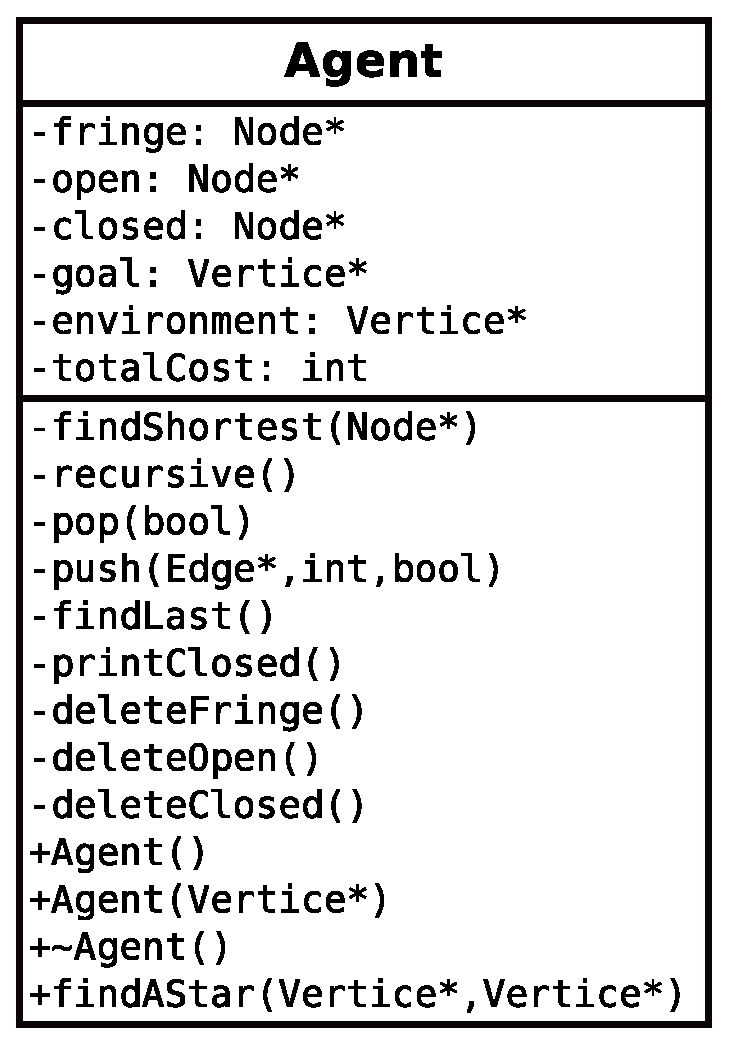
\includegraphics[ width={0.35\textwidth} ]{pictures/uml_agent.eps}
\caption{Description of the A* graph search agent}
\label{fig:uml_agent_graph}
\end{figure}

The agent contains, as shown on the figure \ref{fig:uml_agent_graph}, the following fields:\\
\begin{description}
\item[Fringe:]Open list used in the heuristic, for which we use the shortest path algorithm. The fringe is a pointer to a list of Node, 
a struct described in agent.h and on the picture.
\item[Open:]Open list used in the A* algorithm. It's also a list of Nodes like the fringe.
\item[Closed:]Closed list used to store the final path to the goal. As the Open list and the fringe the closed list is a list of struct Node.
\item[Goal:]Pointer to the goal vertice, is used for compairesons during the hole A* algorithm.
\item[Environment:]Pointer to the beginning of the vertice list. It contains the  environment and is used constantly.
\end{description}

To make the agent be able to execute the A* algorithm we created some helper functions:\\

\begin{description}
\item[findShortest:]Function used to calculate the heuristic value for the A* graph search. Recursivly it stacks values in the Fringe 
and pops from there, until it finds the goal. It gives the total cost of the shortest path in return. It executes recursivly be making a call 
to itself poping the next element in the fringe.
\item[pop:]Funtion that returns the last element in the fringe or the open list, depending on the value of the parameter mode. After 
taking the Node out of the list the list pointer is moved frontwords to the next most probable value.
\item[push:]Function that puts new elements in the lists, it aranges it acording to the cost field int the Node struct. Depending on the 
value provided in the mode parameter the function stores the new element in the fringe or in the open list.
\item[recursive:]Recursive function for calculating the A* graph search algorithm.
\end{description}


\begin{figure}[h]\centering
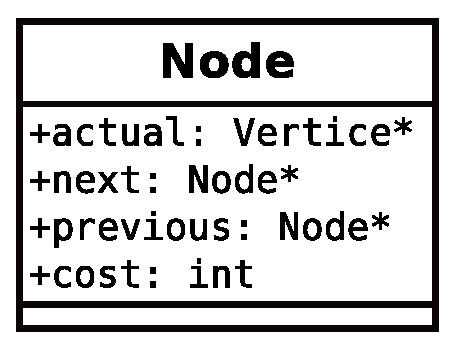
\includegraphics[width=0.35\textwidth]{pictures/uml_node}
\caption{Node structure for list implementation}
\label{fig:node}
\end{figure}


The lists are implemented from the structure Node, see figure \ref{fig:node}. This structure olnly contains the fields:
\begin{description}
\item[Vertice* actual] the vertice pointer that will be used to know the position.
\item[Node* next] next node in the list
\item[Node* previous] is a double linked list, so it has links to the previous nodes.
\item[Int cost] cost of the path to the actual vertice.
\end{description}

\section{A* Star Graph Search algorithm}
The A* graph search implementation is described in this section. It's implemented as a recursive function.\\ 
\begin{description}
\item[The first step] will be to find the heuristic value of the shortest path. This value is calculated with the shortest path algorithm. 
Once we have this value we will use it to make the decissions. We calculate the heuristics this way but the program will be working also 
with other heuristic values.
\item[Second] we add all the edges to the open list making the list longer and will make the program able to move forward.
\item[Third] and last, the program will call itself poping a new element from the open list. If the poped elementis the goal the program 
will finish. 
\end{description}


	
\chapter{Task C}
This is the explanation of the different terms listed below, our results for
this is listed below in their respective sections.
\begin{description}
\item[Completeness:			]
	If there exists a goal state, will the agent find it during runtime?
\item[Optimality:				]
	Wheter the solution the agent finds is in fact the optimal path from A to B.
\item[Time Complexity:	]
	How long it will take for the agent to find the goal, if any.  We are
	measuring this in the following manner -- \textit{How many lines of codes is
	being executed during runtime}.  This is because it will yield a common value
	not influenced by CPU-time and inaccurate clock measurments.
\item[Memory Complexity:]
	How much memory is required by the program to find the solution. We measure
	this using Valgrind to compute how much memory is being used by the program.
\end{description}

\section{A* Tree Search}
\begin{description}
\item[Completeness:			]
\item[Optimality:				]
\item[Time Complexity:	]
\item[Memory Complexity:]
\end{description}

\begin{table}[h]
\centering
\begin{tabular}{	p{0.1\textwidth} p{0.1\textwidth} 
									p{0.2\textwidth} p{0.2\textwidth} }\hline
	Start & End & Time & Tot Memory \\\hline
	1		&	24 	& 	&	\\
	24	&	1 	& 	&	\\
	10	&	5 	& 	&	\\
	5		&	10 	& 	&	\\
	1		&	20 	& 	&	\\
	20	&	1		&		&	\\
\end{tabular}
\caption{Measured values for A* Tree Search}\label{tbl:sumTree}
\end{table}

\section{A* Graph Search}
\begin{description}
\item[Completeness:			]
\item[Optimality:				]
\item[Time Complexity:	]
\item[Memory Complexity:]
\end{description}

\begin{table}[h]
\centering
\begin{tabular}{	p{0.1\textwidth} p{0.1\textwidth} 
									p{0.2\textwidth} p{0.2\textwidth} }\hline
	Start & End & Time & Tot Memory \\\hline
	1		&	24 	& 	&	\\
	24	&	1 	& 	&	\\
	10	&	5 	& 	&	\\
	5		&	10 	& 	&	\\
	1		&	20 	& 	&	\\
	20	&	1		&		&	\\
\end{tabular}
\caption{Measured values for A* Graph Search}\label{tbl:sumGraph}
\end{table}





	
\chapter{Task D}
\section{Dynamic environment}

\subsection{Full sensing}
With full sensing the agent can move continously and recalculate the optimal
path when an environment change occurs. Since fully senses the environment it
will take any obstructions into account when calculating the optimal path and
next move. Therefore it will not hit any objects and continously move around
paths that are obstructed.


\subsection{Partial Sensing}
When the agent senses or encounters an obstruction it must stop and retreat to
the previous Vertice or stay on the current Vertice. Then it has to update the 
environment and re-calculate the optimal path to decide which move to make next.

\subsection{No waypoint addition}
The inability to create new Vertices and Edges will hinder the possibility of
discovering a shortcut to a Vertice or an intermediate vertice between two
vertices.  This might result in a complete halt in the graph traversal or
inability to find a result at all.

If e.g one has a map of an area and it contains an articulation point. If this
articulation point is obstructed one is not able to traverse the graph. If one
has the ability to discover and add new edges and vertices one might find an
edge or vertice that connects the two sub graphs and avoids the articulation
point all together.

Another reason why it would cause a problem is if a NPC in a game has a blocked
path in the environment which is later unblocked. Inability to update this and
add a new vertice and edge to the environment will make it unable to traverse
this way, in which case it would come to a halt and gameplay would be much
worse.

In this case it would make sense to have the possibility of adding additional
edges and vertices.  If however the task is to find the optimal path in the
current environment it wouldn't make sense to have this ability.






	
\chapter{Task E}
\section{Change management}
The bots have multiple ways of sensing the environment. An NPC will initially
receive the whole environment of static objects in the environment; houses,
structures and un-movable objects.  Based on this it plot its course and then
maintain an partially observable environment of a perimeter around itsself.

In this perimeter the NPC will be able to sense changes as they happen. Any
object entering the NPC's perimeter will bew added to its memory when they
are sensed through viewing.

Other live objects will be implemented into the environment as they are seen
and if they are touched without viewing them, i.e backing into a crate/wall or
being attacked).

Once they move out of the NPC's perimeter they will be removed from its memory
and then re-appear when they re-enter its perimeter.

\section{Methods of sensing}
The NPC's methods of sensing that an object appears in its path is through the
environment that depicts all static objects, and that the NPC receive a
specified environment from the server during gameplay about where it is and what
is in its personal perimiter.

Based on this the static objects will be avoided from the start, but dynamic
changes will be updated when they enter the NPC's perimiter.  Either through
touch or viewing.




	
	\chapter{Run instructions}
		Our code is separated into two different programs. The main.cpp will run the
		tree search algorithm and the graphSearch.cpp will run the graph search
		algorithm.

		On windows the file path has to be altered to "../vertice.lst" instead of
		"vertice.lst" or similar according to where it is located in relation to
		where the executable is located.

		In visual studio import all files to the project and build and run either
		graphSearch.cpp or main.cpp to test the software.

		On linux run "make" to compile the tree search algorithm. Then execute 
		"./run.exe" to test the program.

		Use "make graph" to compile the graph search algorithm. Then also execute
		"./run.exe" to the the program.  
		
		To measure the memory allocation and so on run "valgrind ./run.exe" in
		terminal to run it, and on program exit it will display the memory usage.

\end{document}

